\chapter{项目背景}

随着机器人技术的发展,机器人的应用场景越来越多。但是目前自动控制机器人尚不能执行多数复杂任务,特别是抢险救灾等需要随机应变的任务,这种情况下需要遥操作机器人。目前机器人远程控制普遍采用手柄(如图~\ref{panal})或键盘控制方式,且监控方式普遍为摄像头图像显示在监视器上,与现场操作差别很大。


\begin{figure}[htbp]
\centering
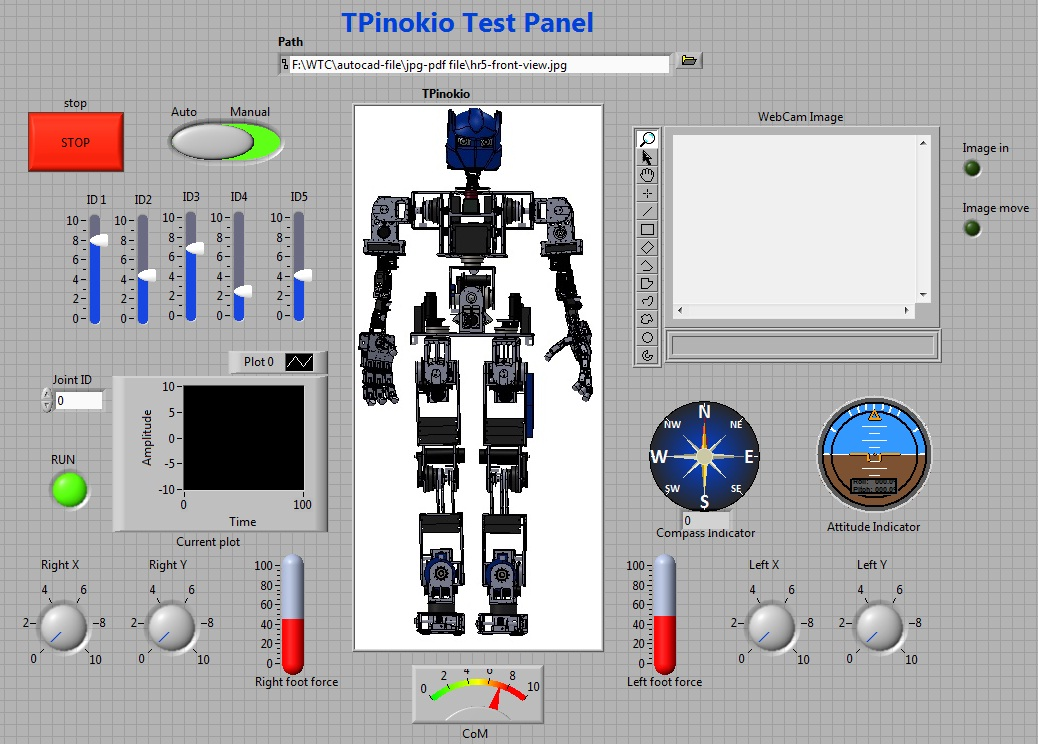
\includegraphics[width=10cm]{CtrlPanel.jpg}
\caption{机器人控制面板} 
\label{panal}
\end{figure}

现有的基于动作捕捉的遥操作系统如OptiTrack和机械外骨骼等,虽然用户体验很好,但是成本极高,依赖性强,无法大规模应用。

现有的实时VR显示大多基于图像拼接,图像采集设备昂贵,实时性和图像质量无法同时兼顾,且对算力要求很高。

本作品提出了一种廉价、低延时的遥操作系统,其双目摄像头及VR显示系统可使操作者看到具有立体感的实时画面,手持追踪器操作机械臂末端符合人类日常使用手进行操作的习惯,可以给予操作者以身临其境的操作体验。


\chapter{现有系统问题}

\section{现有的三维图像采集系统}

目前三维场景重构需要很高的算力,分辨率低且不能保证实时性,目前较成熟的实时三维场景采集系统基本上都基于图像拼接技术:

\begin{figure}
\begin{minipage}{0.48\textwidth}
  \centering
  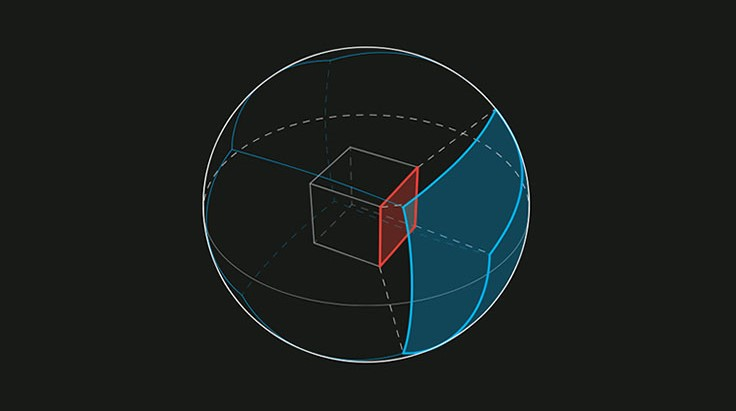
\includegraphics[height=4cm]{Cube.jpg}
  \caption{立方体拼接}
  \label{cube}
\end{minipage}\hfill
\begin{minipage}{0.48\textwidth}
  \centering
  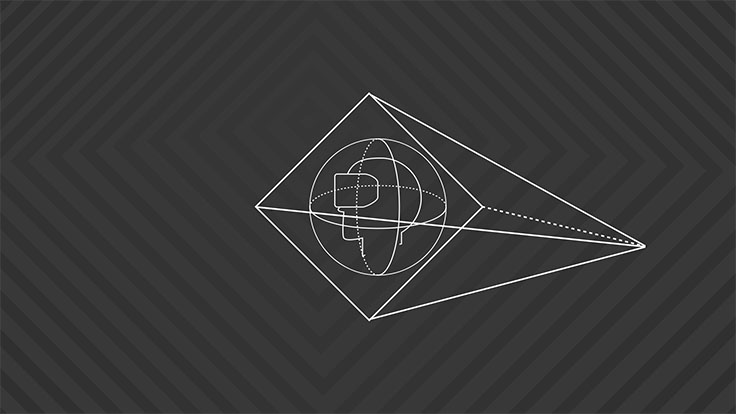
\includegraphics[height=4cm]{Tri.jpg}
  \caption{金字塔形拼接}
  \label{tri}
\end{minipage}
\end{figure}

要创建一个360度全景视频,无论是使用特殊的摄像机同时记录场景,还是将多个不同角度的GoPros图像拼接在一起,传入的每个视频文件分辨率是4K和更高,总比特率会超过50 Mb/s。而用于VR的360度视频的比特率是其两倍,即每小时44 GB视频。如果要实时发送和接收这些图像信息,对带宽等网络环境要求非常高。拼接这些图像则会消耗大量的算力,无论是采用立方体(见图~\ref{cube})还是金字塔形拼接方式(见图~\ref{tri})。因此,运算和传输延迟加起来会达到2s以上,实时性和图像质量无法同时兼顾。

以Google Jump(见图~\ref{jump})为例,Google Jump使用24个GoPro,环绕一个圆形分布,考虑到GoPro单个相机的价格(2000-3000人民币)上述系统造价非常昂贵。

\begin{figure}[htbp]
\small
\centering
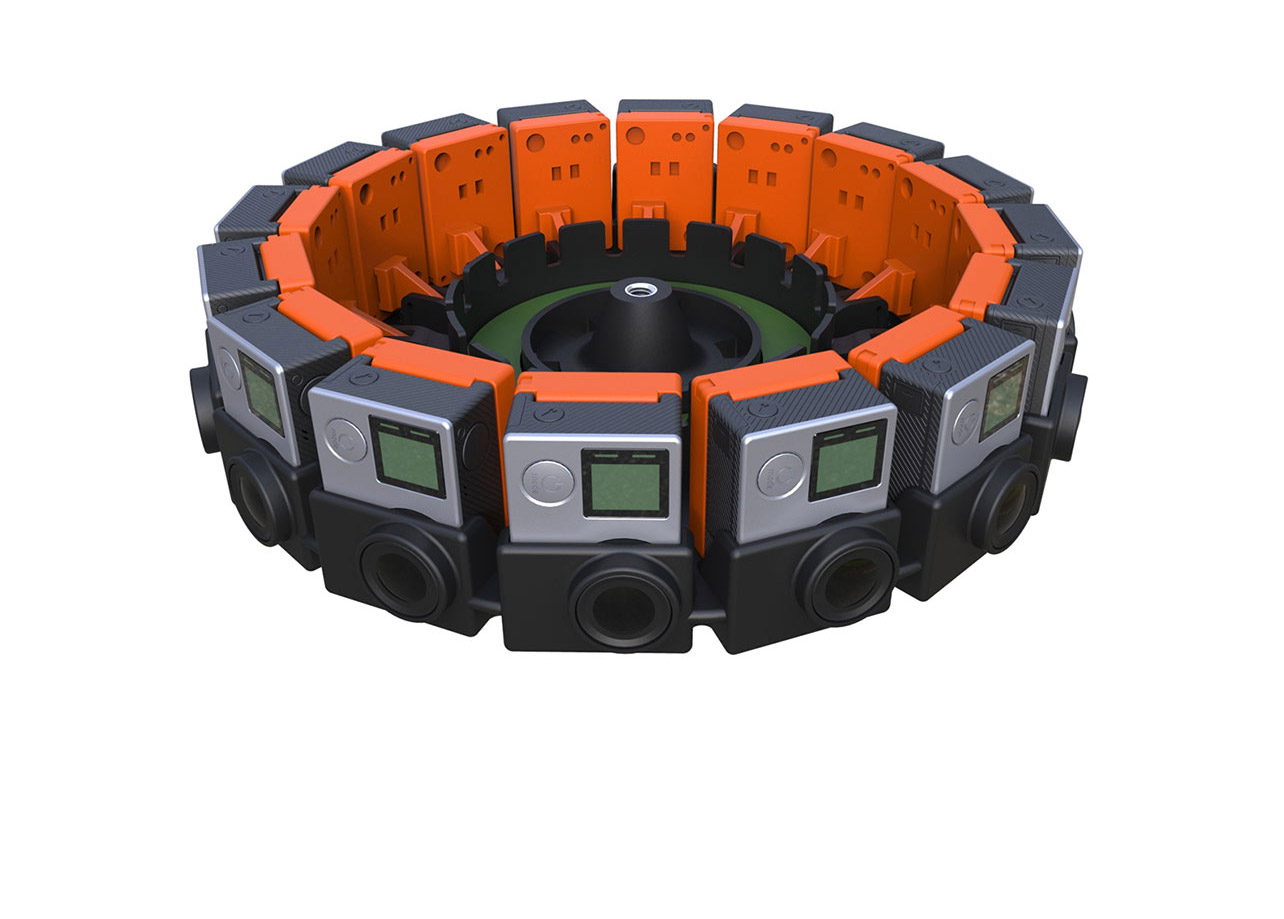
\includegraphics[width=16cm]{google-jump.jpg}
\caption{Google Jump} 
\label{jump}
\end{figure}

\section{现有的机器人遥操作系统}

\subsection{计算机指令或手柄控制}
许多需要人工远程操控的机器人,其操作方式是向控制面板或计算机输入指令而实现。通常情况下,因为机器人自由度很多,常需要事先编好一系列的动作,使用指令调用。

手柄常用来控制一些自由度较低的系统,如机械臂,多数是直接控制各关节电机转速,从而实现机械臂控制。

这些传统的远程控制方式对操作者要求很高,操作者需要实现接受一系列培训及练习,以熟悉操作平台其交互体验不是很理想。

\subsection{OptiTrack动作捕捉系统}
OptiTrack\footnote{\url{http://optitrack.com/}} (见图~\ref{opti})是基于一系列红外摄像机的动作捕捉系统解决方案,在操作者身上贴多个感光球,通过四周的十多个红外摄像机来计算每一个感光球的位置,从而获得人的动作数据。
\begin{figure}[H]
\small
\centering
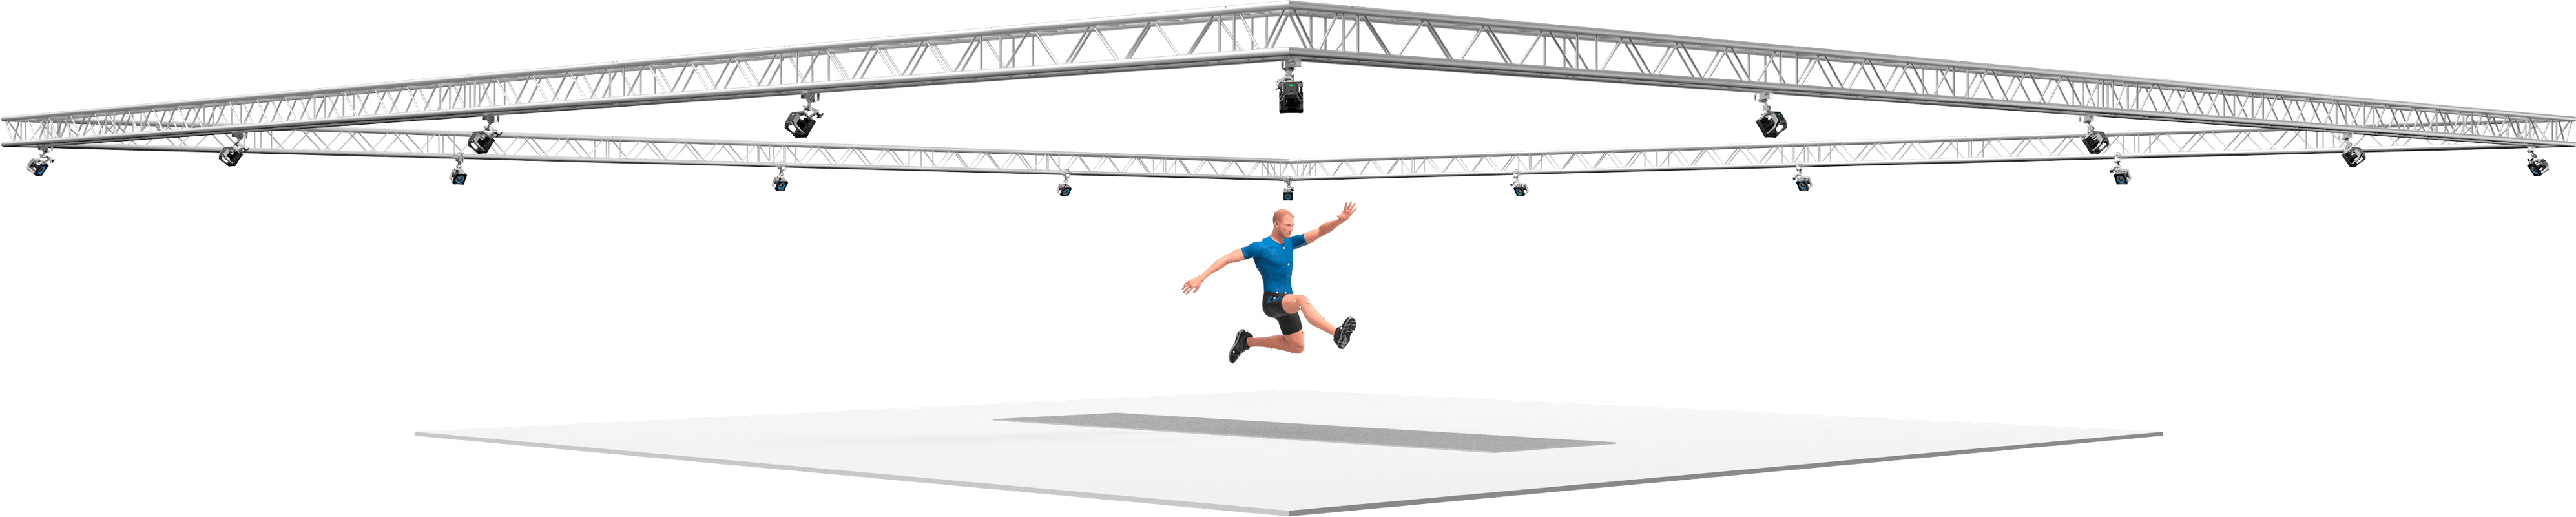
\includegraphics[width=16cm]{movementPrime41_16.png}
\caption{OptiTrack} 
\label{opti}
\end{figure}
由于此解决方案需要至少12个高速红外摄像机和配套的处理系统,而一个红外摄像机售价4000-5000美元,整个系统的成本非常高,用其做机器人控制并不现实。

\subsection{T-HR3人形机器人遥操作系统}

T-HR3(如图~\ref{thr})是一种远程机动系统,它通过外骨骼和数据手套将手,手臂和脚部动作映射到机器人。

就操作者近端方面而言,T-HR3采用机械外骨骼加上双手的数据手套。由于机械外骨骼以力信号作为控制端的输出信号,所以,机械外骨骼和操作者之间本身就存在一定的滞后性,而且,力信号易受外力干扰,所以存在信号不稳定的问题。

更重要的是,T-HR3需要一套昂贵且笨重的外骨骼,其应用场景十分受限。

\begin{figure}[htbp]
\small
\centering
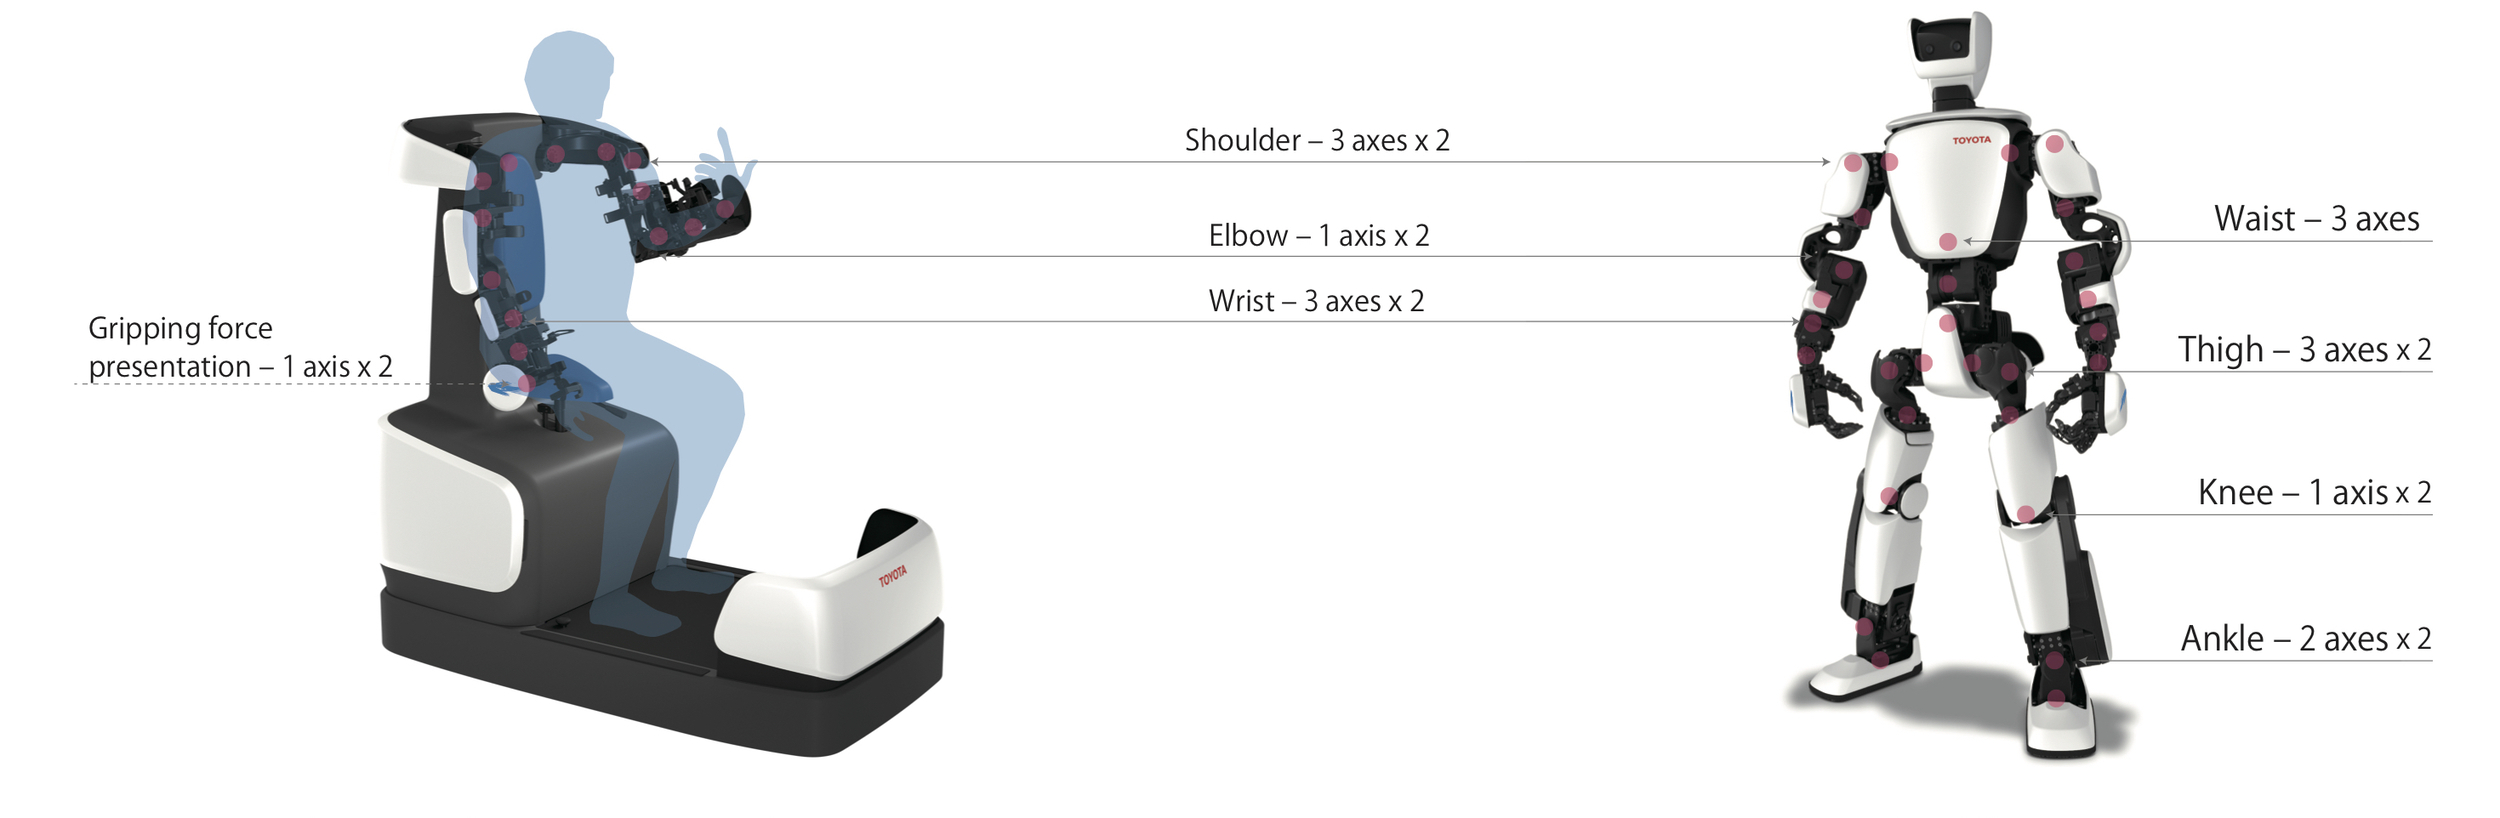
\includegraphics[width=16cm]{T-HR3_2.jpg}
\caption{T-HR3} 
\label{thr}
\end{figure}




\chapter{系统简介}
本作品\footnote{本章节内独创内容均已申请实用新型专利,国家知识产权局电子申请案卷编号:274278199}
旨在解决现有机器人遥操作系统的上述问题,提出了一套低成本、操作简单、实时性好、可提高用户体验的遥操作解决方案。


\begin{figure}[htbp]
\small
\centering
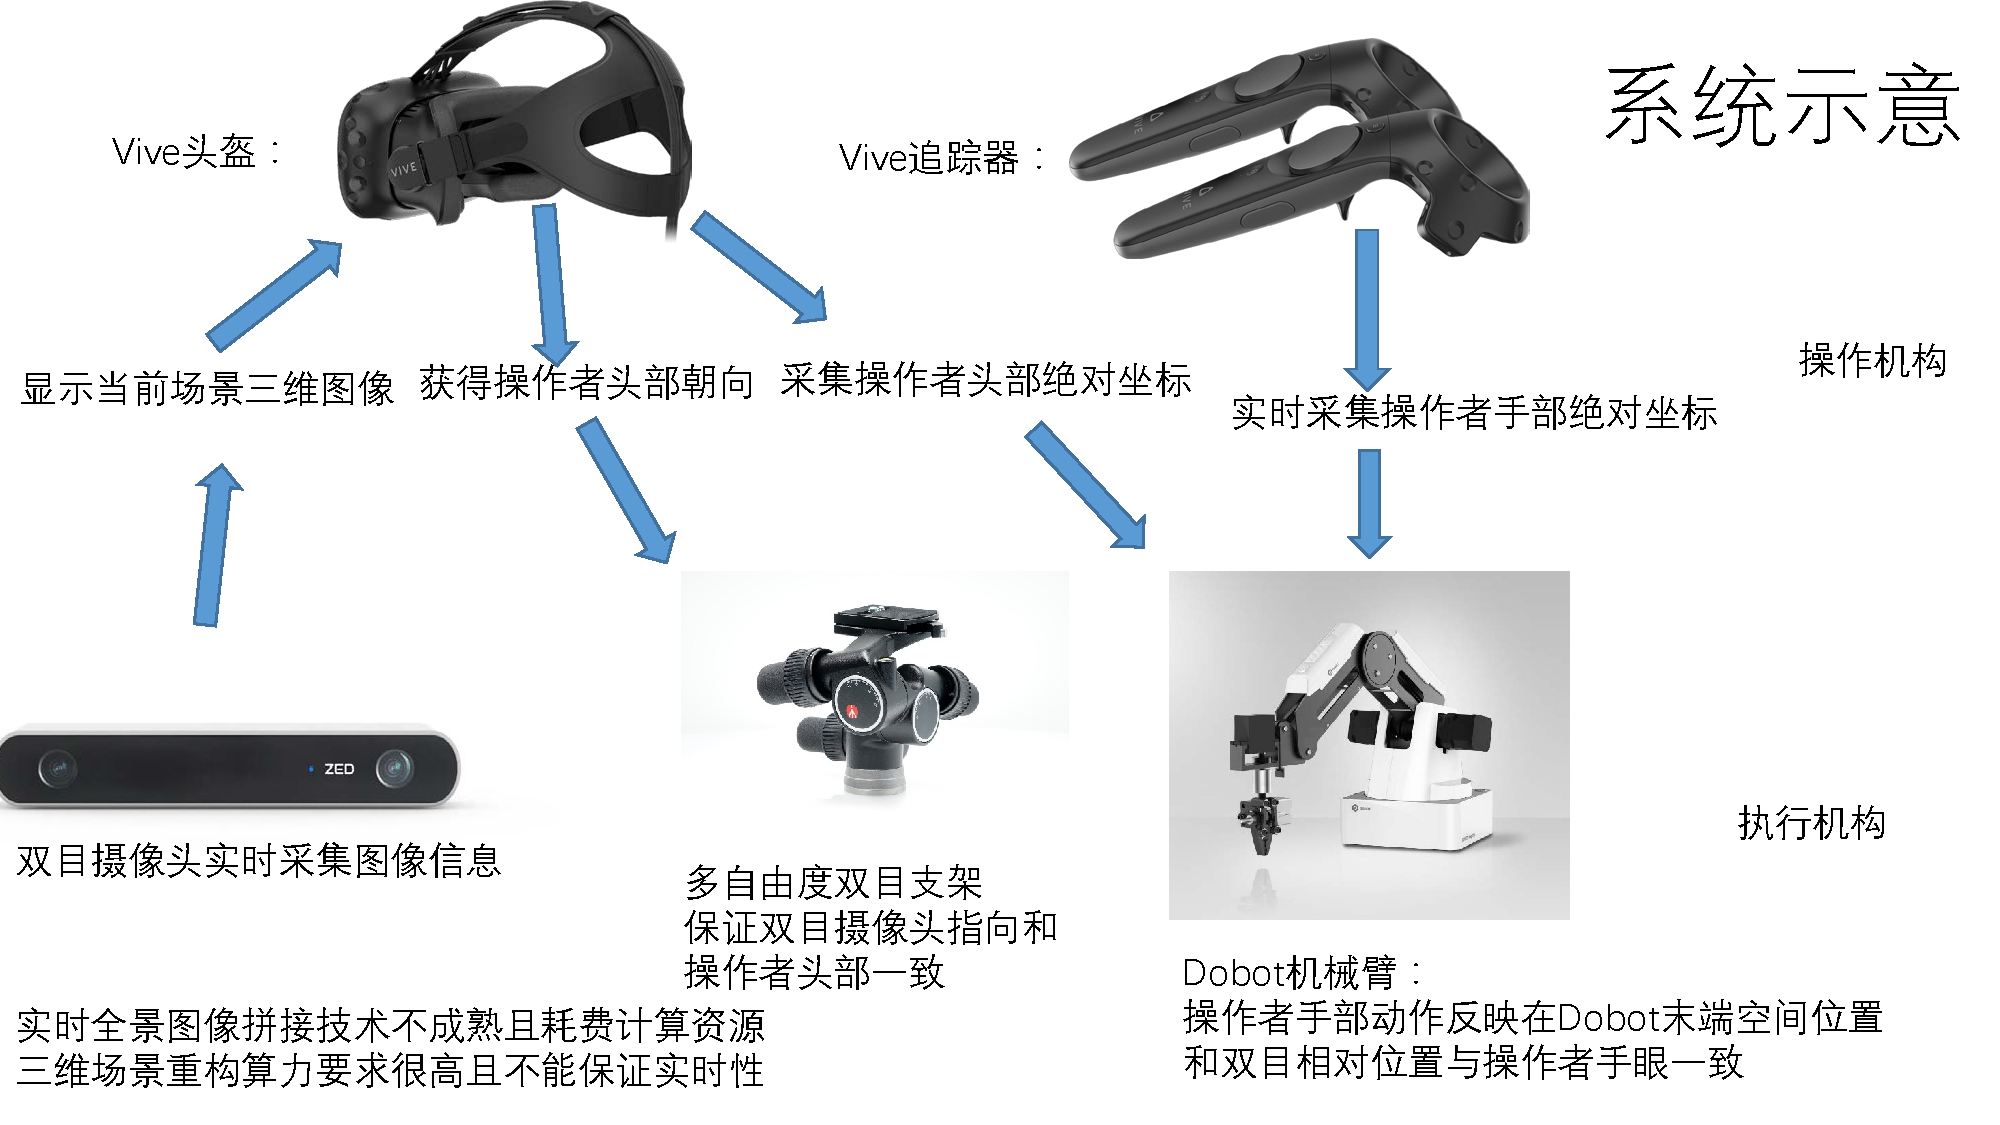
\includegraphics[width=16cm]{pic.pdf}
\caption{系统示意} 
\label{pic}
\end{figure}


如图~\ref{pic}所示:

我们采用双目摄像头采集实时场景信息,两个目采集到的图像对应到VR眼镜的两个显示屏中,同时多自由度双目支架保证双目朝向和操作者双眼朝向一致,从而简单的使操作者可以看到实时的立体场景,同时降低了成本、减小了延迟。

虚拟现实头盔和追踪器上的红外定位模块精确的确定了它们的绝对位置,由此可得它们的相对位置,我们可以使机械臂末端和双目摄像头的相对位置和其一致,从而实现操作者直接用手的位置来控制机械臂。


该项目可分为两个子系统:图像显示系统及机器人控制系统。
	
	\section{VR远程监视系统}
本系统旨在提供一个具有较强立体感的实时全景图像,并解决现有系统的问题以及最大化的降低造价,以使远程操控者获得身临其境的体验。我们用ZED双目摄像头来采集实时场景信息,两个目采集到的图像对应到VR眼镜的两个显示屏中,而搭载ZED的多自由度舵机支架可随操纵者头部的转动而实时旋转,以保证双目摄像头的朝向和操作者双眼朝向一致,从而使操作者可以实时地看到各方位的立体场景。
	
此系统硬件部分仅由一个双目摄像头,转台,虚拟现实头盔组成,成本低,且部件较常见。双目摄像头可以由两个独立的摄像头替代,只需保证两摄像头间距和瞳距相似即可,随着虚拟现实技术的发展,分辨率较高的Vive VR头盔(如图~\ref{vivevr})价格可以为普通人所接受,Google Cardboard(如图~\ref{card})售价则低至10RMB,需要和智能手机配合使用。
\begin{figure}
\begin{minipage}{0.48\textwidth}
  \centering
  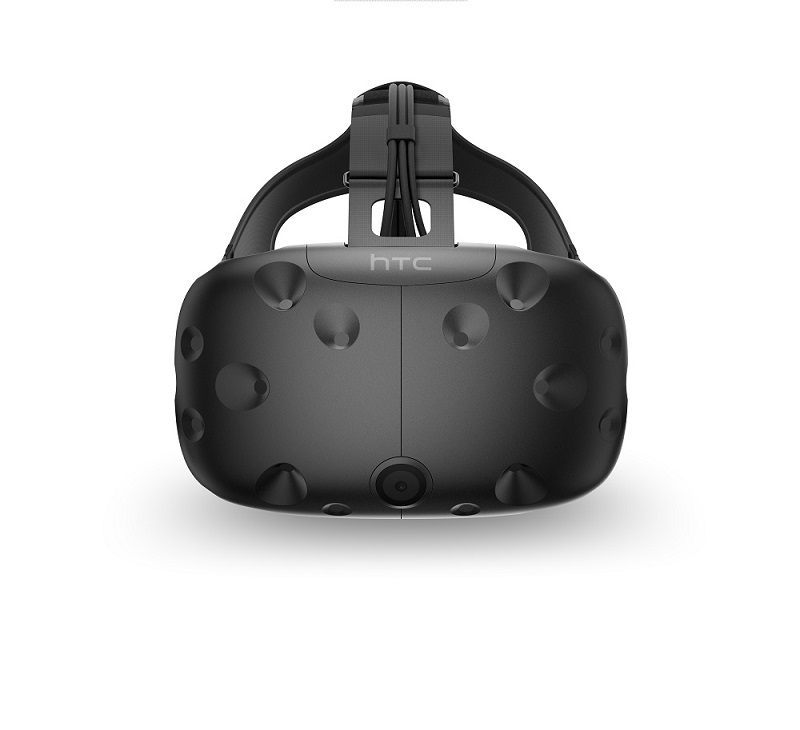
\includegraphics[height=4cm]{HMD.jpg}
  \caption{Vive VR头盔}
  \label{vivevr}
\end{minipage}\hfill
\begin{minipage}{0.48\textwidth}
  \centering
  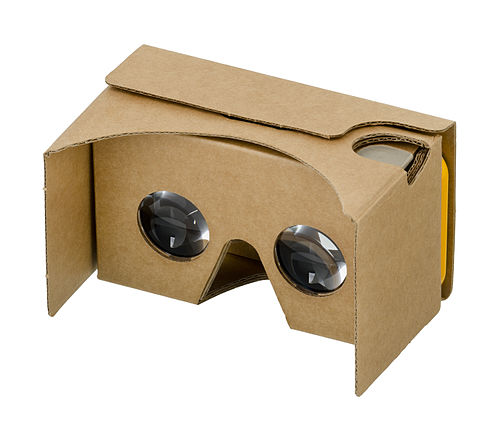
\includegraphics[height=4cm]{Google-Cardboard.jpg}
  \caption{Google Cardboard}
  \label{card}
\end{minipage}
\end{figure}

因为只需要传输两个摄像头的图像,并不需要复杂的运算,这套机械式的实时全景系统延迟很小。

\section{Vive追踪器遥操作系统}

虚拟现实头盔和追踪器上的红外定位模块精确的确定了它们的绝对位置,由此可得它们的相对位置,我们可以使机械臂末端和双目摄像头的相对位置和其一致,从而实现操作者直接用手的位置来控制机械臂。

此系统使得操作者能够利用自身的动作控制机器人的运动,符合人类的行为习惯,因而会带来良好的操作体验。

Vive虚拟现实套件\footnote{\url{https://www.vive.com/cn/product/}}(如图~\ref{vivekit})包括Vive追踪器,Vive VR头盔和Lighting基站,官网售价5488RMB,远低于OptiTrack或T-HR3外骨骼部分的售价。而这套系统完全可以胜任大多数任务。而且Vive VR套件对环境要求很低,可以随时搭建操作环境。
\begin{figure}[H]
\small
\centering
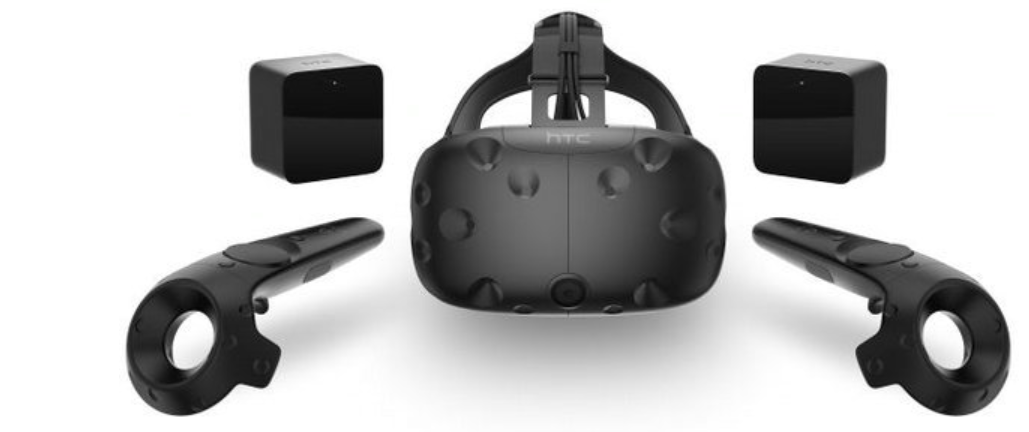
\includegraphics[width=16cm]{vive.PNG}
\caption{Vive虚拟现实套件} 
\label{vivekit}
\end{figure}

\chapter{项目展示}

我们首先完成了实时图像采集与显示系统,调试至观看体验最佳;之后我们研究并改写Dobot指令集,设计并制做了机械臂末端执行机构,读取了Vive坐标,实现用Vive远程控制Dobot,并测试了整套系统;不久前,我们为验证此遥操作系统的可迁移性,用NAO人形机器人替换Dobot,最终完成了这一系统。

下面以时间顺序分阶段介绍我们的成果:

\section{实时图像采集与显示系统}
实现了多自由度机械结构托举的双目摄像头,随着操作者头部的转动而同步转动{\kaishu (参见视频1)},以采集实时图像信息(如图~\ref{zed})。{\kaishu (参见视频2)}在这一阶段,我们的VR平台暂时使用使用Google Cardboard(谷歌折叠式纸板虚拟现实显示器)(如图~\ref{card})。操作者头部姿态数据由其中Android手机自身的陀螺仪获取,并发送到舵机的控制端控制舵机转动。

\begin{figure}
\begin{minipage}{0.48\textwidth}
  \centering
  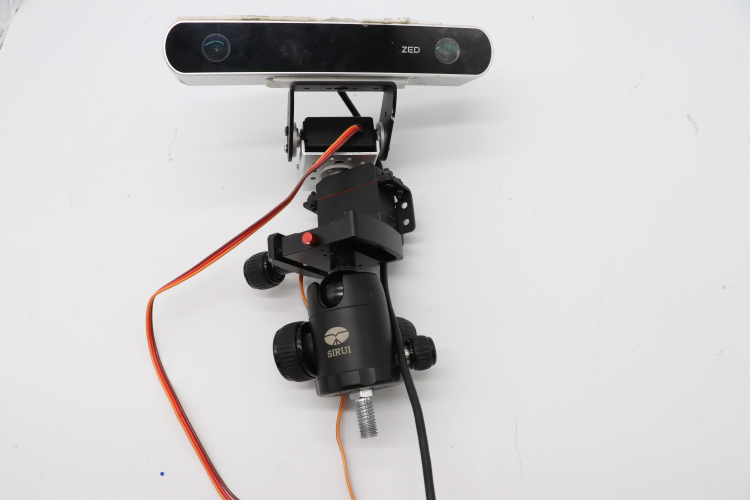
\includegraphics[height=6cm]{ZED0.png}
  \caption{双自由度机械结构托举的双目摄像头}
  \label{zed}
\end{minipage}\hfill
\begin{minipage}{0.48\textwidth}
  \centering
  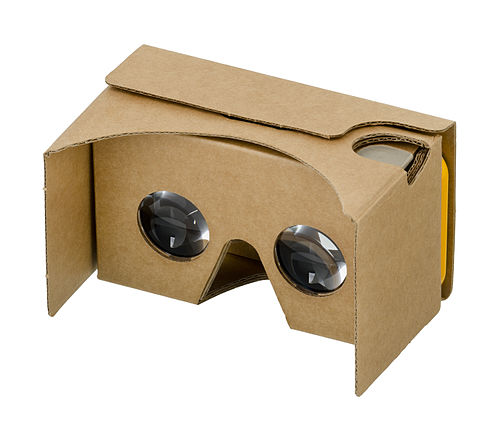
\includegraphics[height=6cm]{Google-Cardboard.jpg}
  \caption{Google Cardboard}
  \label{card}
\end{minipage}
\end{figure}

同时,在这一阶段,我们在机械臂末端加上了吸盘执行机构,使用气泵和电磁阀组建了一个吸附装置(见图~\ref{bump})。

\begin{figure}
\begin{minipage}{0.48\textwidth}
  \centering
  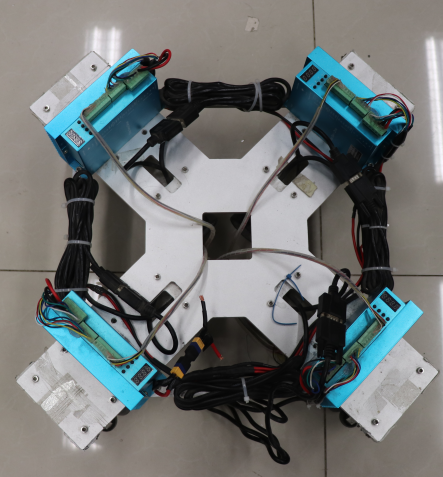
\includegraphics[height=6cm]{car.png}
  \caption{全向轮底盘}
  \label{car}
\end{minipage}\hfill
\begin{minipage}{0.48\textwidth}
  \centering
  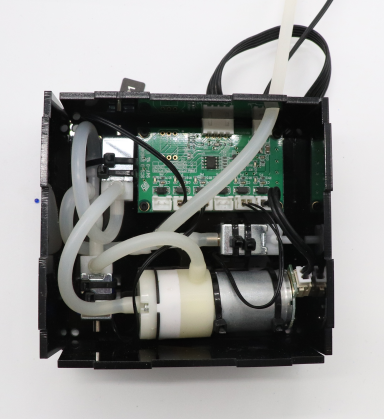
\includegraphics[height=6cm]{bump.png}
  \caption{气泵和电磁阀组建的吸附装置}
  \label{bump}
\end{minipage}
\end{figure}


同时我们改写了DOBOT机械臂底层及接口,解决了串口控制卡顿的问题。实现用遥控器-接收机控制系统,远程完成叠纸杯实验。{\kaishu (参见视频3)}

\section{机械臂遥控与执行机构(Vive+DOBOT机械臂)}

在这一阶段,我们完成了一个由全向轮底盘(如图~\ref{car})移动的机械臂(如图~\ref{sys}),平台上搭载双自由度机械结构托举的ZED摄像头,随着操作者头部的转动而同步转动,以采集实时图像信息。我们将上一阶段的基于Google Cardboard的系统迁移到了Vive虚拟现实头盔上,实现了更清晰的显示效果。


\begin{figure}[htbp]
\small
\centering
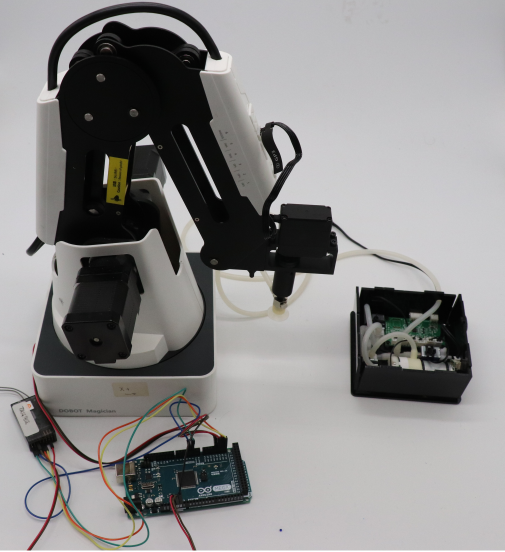
\includegraphics[width=8cm]{Dobot0.png}
\caption{DOBOT机械臂及通讯系统} 
\label{sys}
\end{figure}


我们可以实现读取追踪器和VR头盔绝对位置并通过串口发送。可以看到图~(\ref{POS})中输出了左手,右手和头盔的绝对坐标。我们改写了机械臂底层及接口,解决了串口控制卡顿的情况。{\kaishu (参见视频4及5)}
\begin{figure}[htbp]
\small
\centering
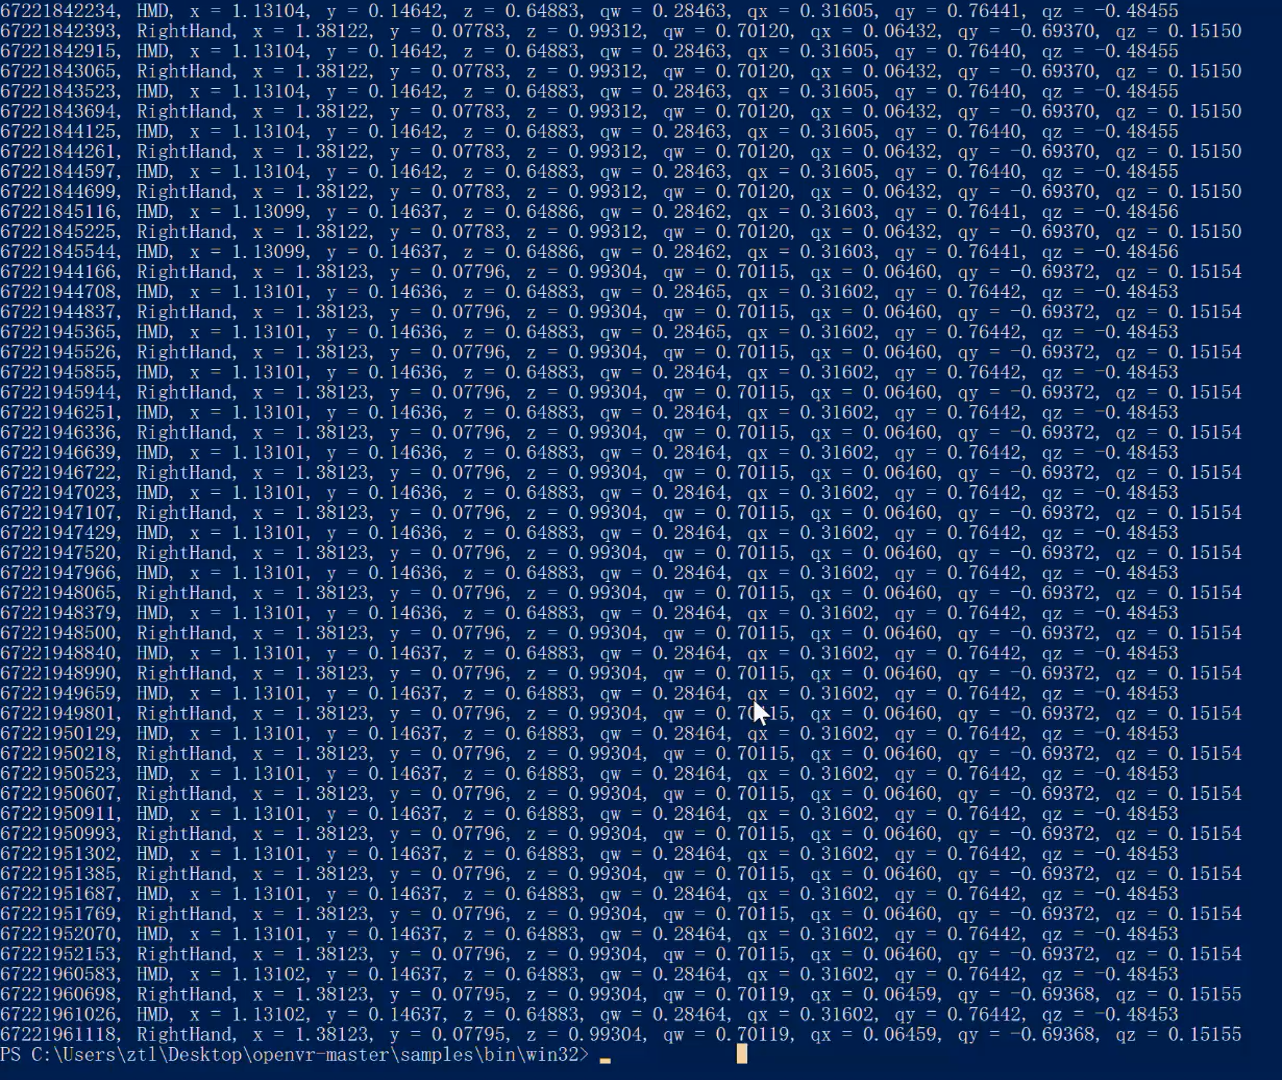
\includegraphics[width=16cm]{Date.png}
\caption{追踪器和VR头盔绝对位置} 
\label{POS}
\end{figure}

从而实现了用Vive追踪器远程控制机械臂,为了测试机械臂的响应,我们用Vive追踪器操控Dobot机械手在竖直平面内画一个五角星{\kaishu (参见视频6)}

之后,我们使用上述双目摄像头系统和Vive配合,远程完成了叠纸杯实验(图~\ref{cup})。{\kaishu (参见视频7)}

\begin{figure}[htbp]
\small
\centering
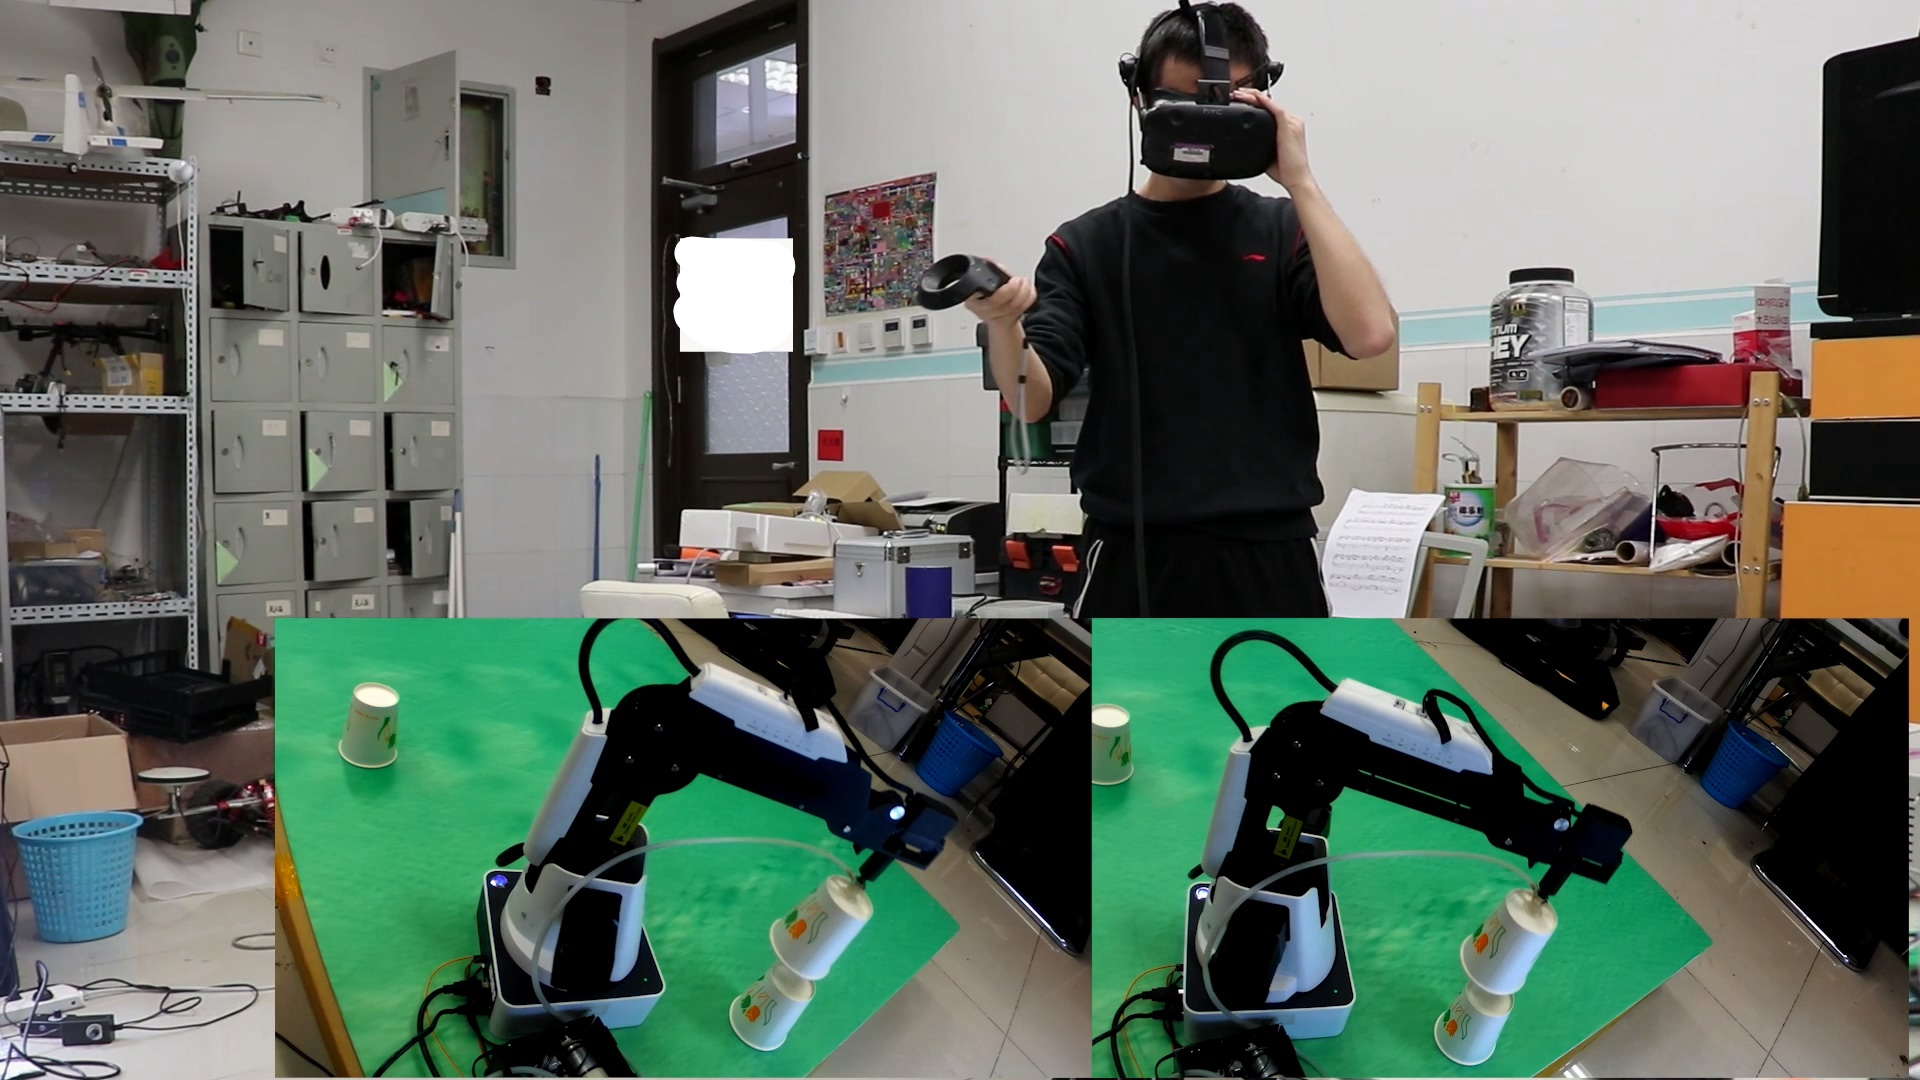
\includegraphics[width=10cm]{vivedobot.jpg}
\caption{DOBOT远程叠纸杯实验} 
\label{cup}
\end{figure}


\section{机器人遥控与执行机构(NAO人形机器人)}

为说明此系统的普适性,我们将此系统成功拓展到机械结构与Dobot差别很大的NAO人形机器人上,用追踪器控制机器人手臂的运动(图~\ref{8NAO})。\footnote{由于NAO自身设计的缺陷(易失去平衡),我们现阶段并没有加入腿部动作,且将手臂动作对称处理}成功完成Vive远程控制NAO的实验。{\kaishu (参见视频8)}

\begin{figure}[htbp]
\small
\centering
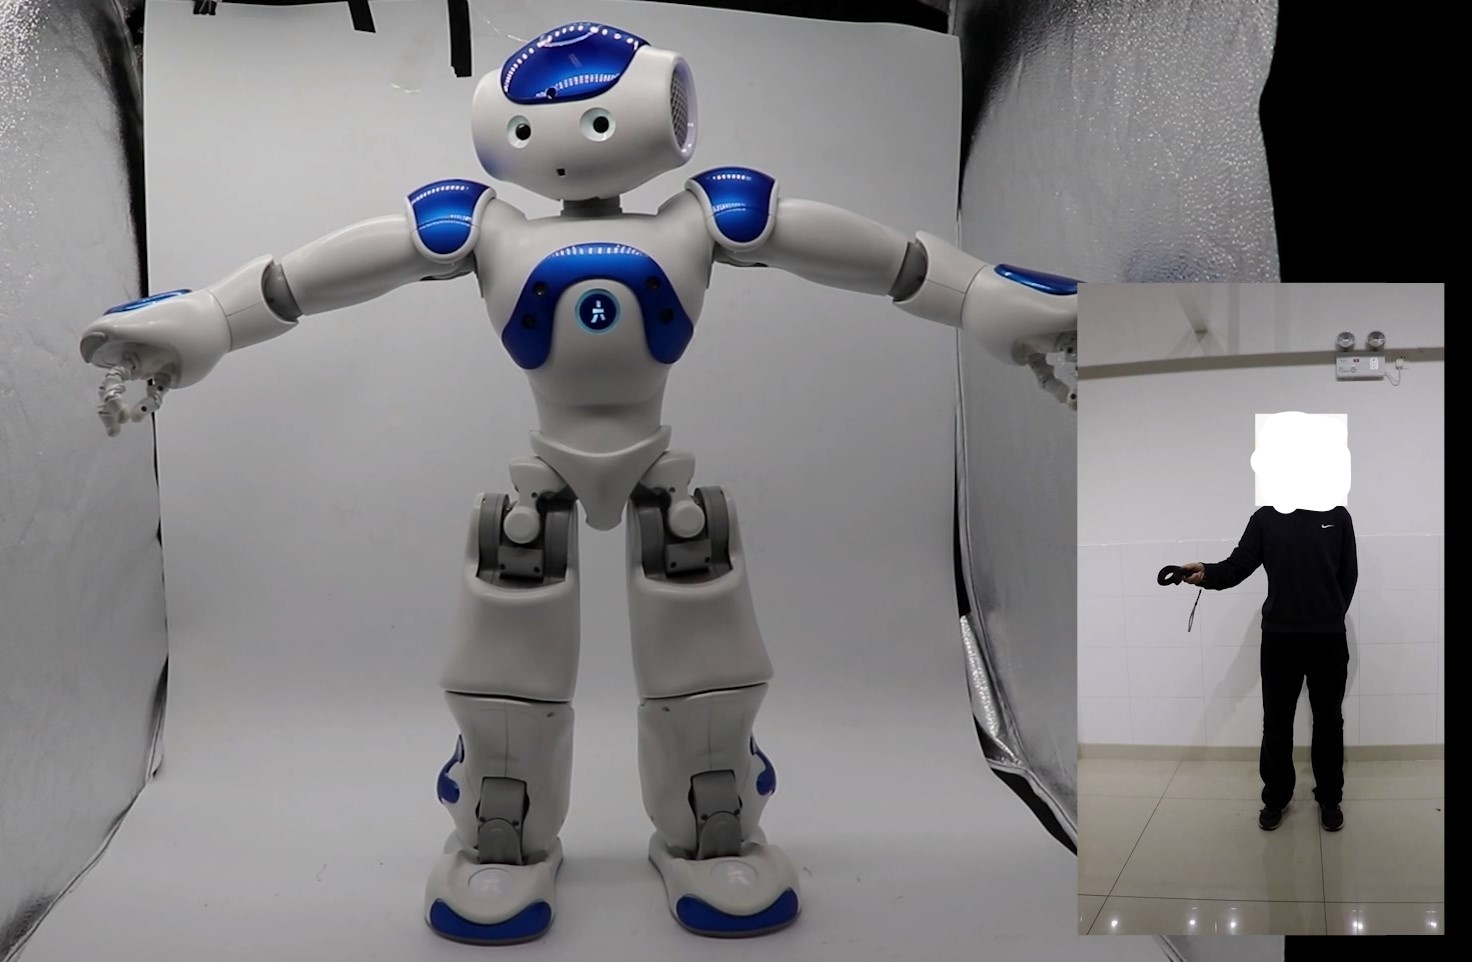
\includegraphics[width=10cm]{8NAO.jpg}
\caption{Vive远程控制NAO} 
\label{8NAO}
\end{figure}


\section{总结}

经以上测试,我们这套系统远程控制实时性很好,视频传输及控制延迟小于200ms,在VR眼镜中有很强的立体感,操作简单,且方便迁移至其他系统。



\chapter{技术细节}

此系统实现了远程操作的完整功能,整个系统硬件层面架构和数据流向分别如图~\ref{stru}和~\ref{logic}所示

\begin{figure}[htbp]
\small
\centering
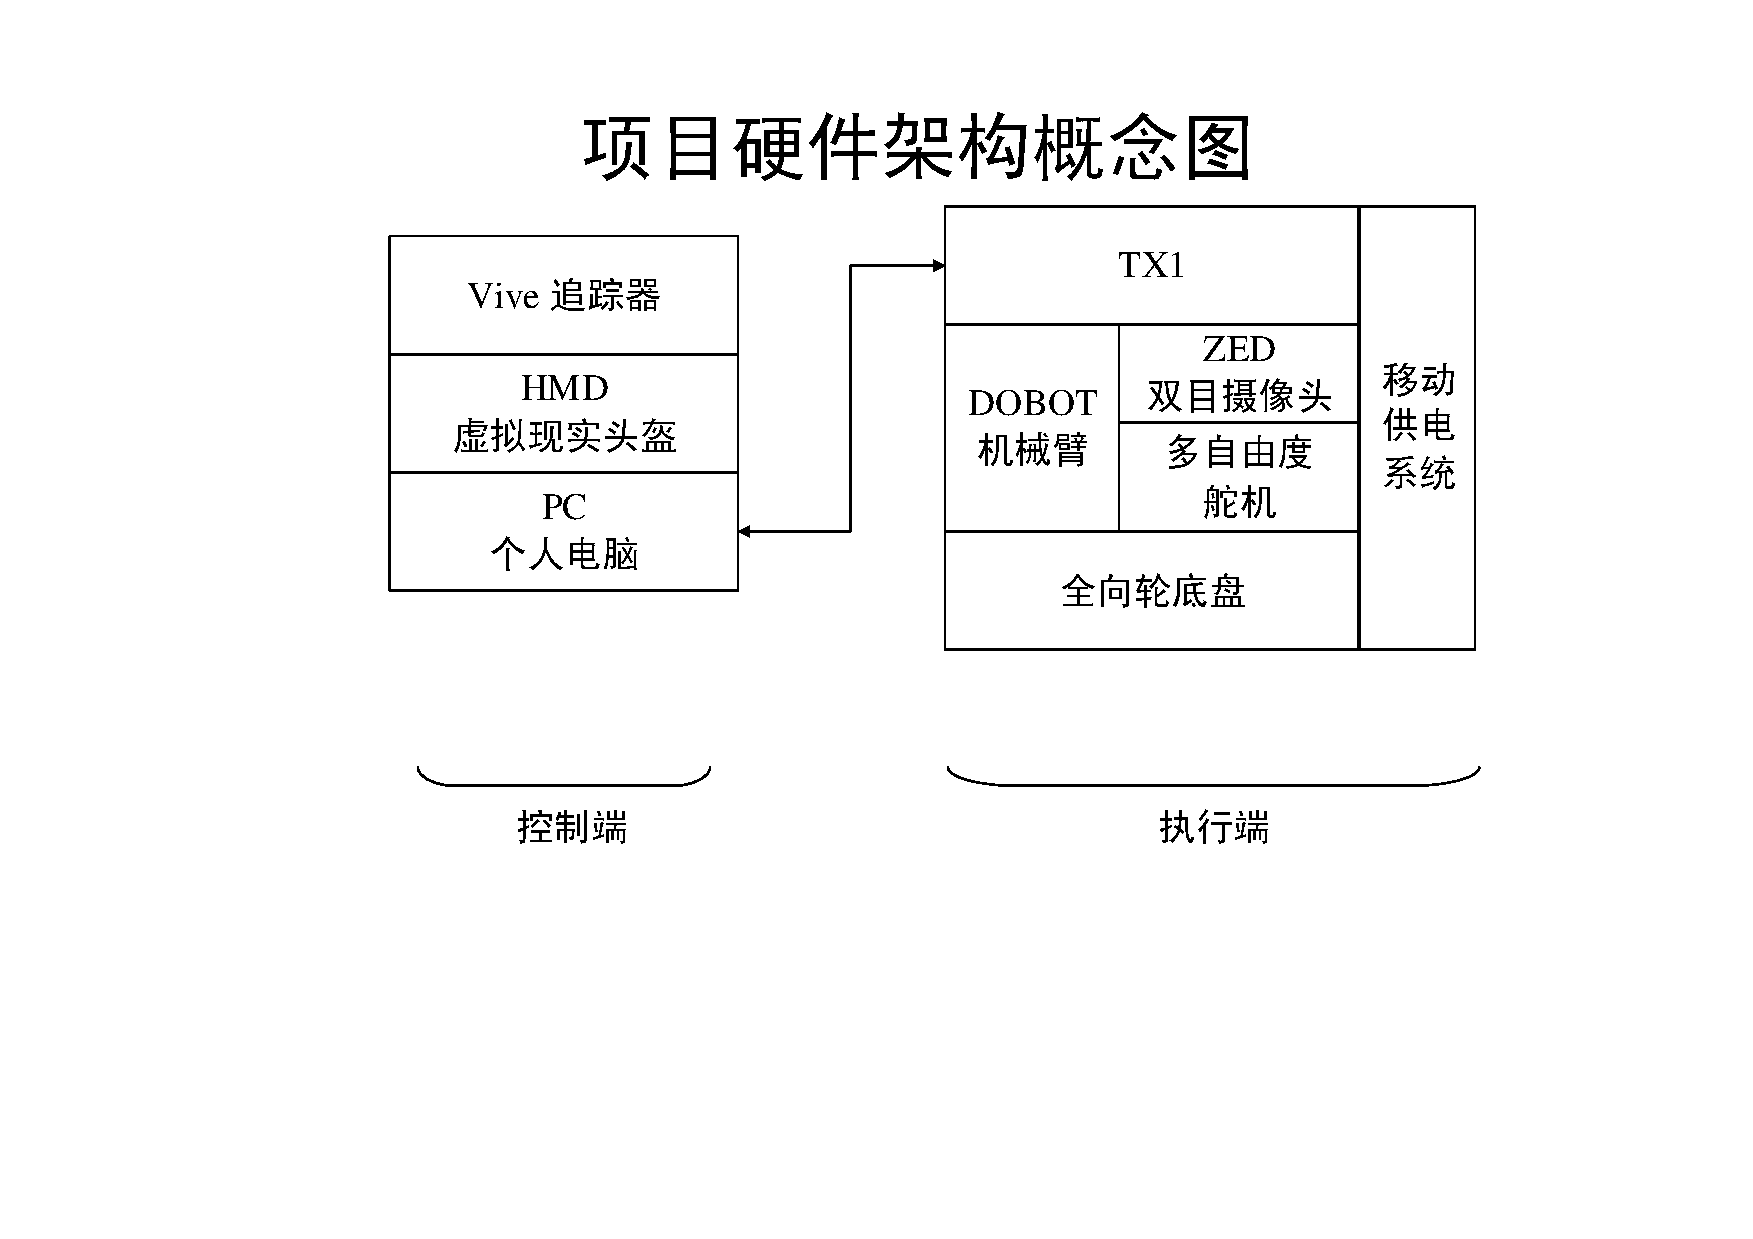
\includegraphics[width=12cm]{stru.pdf}
\caption{硬件架构总览} 
\label{stru}
\end{figure}

\begin{figure}[htbp]
\small
\centering
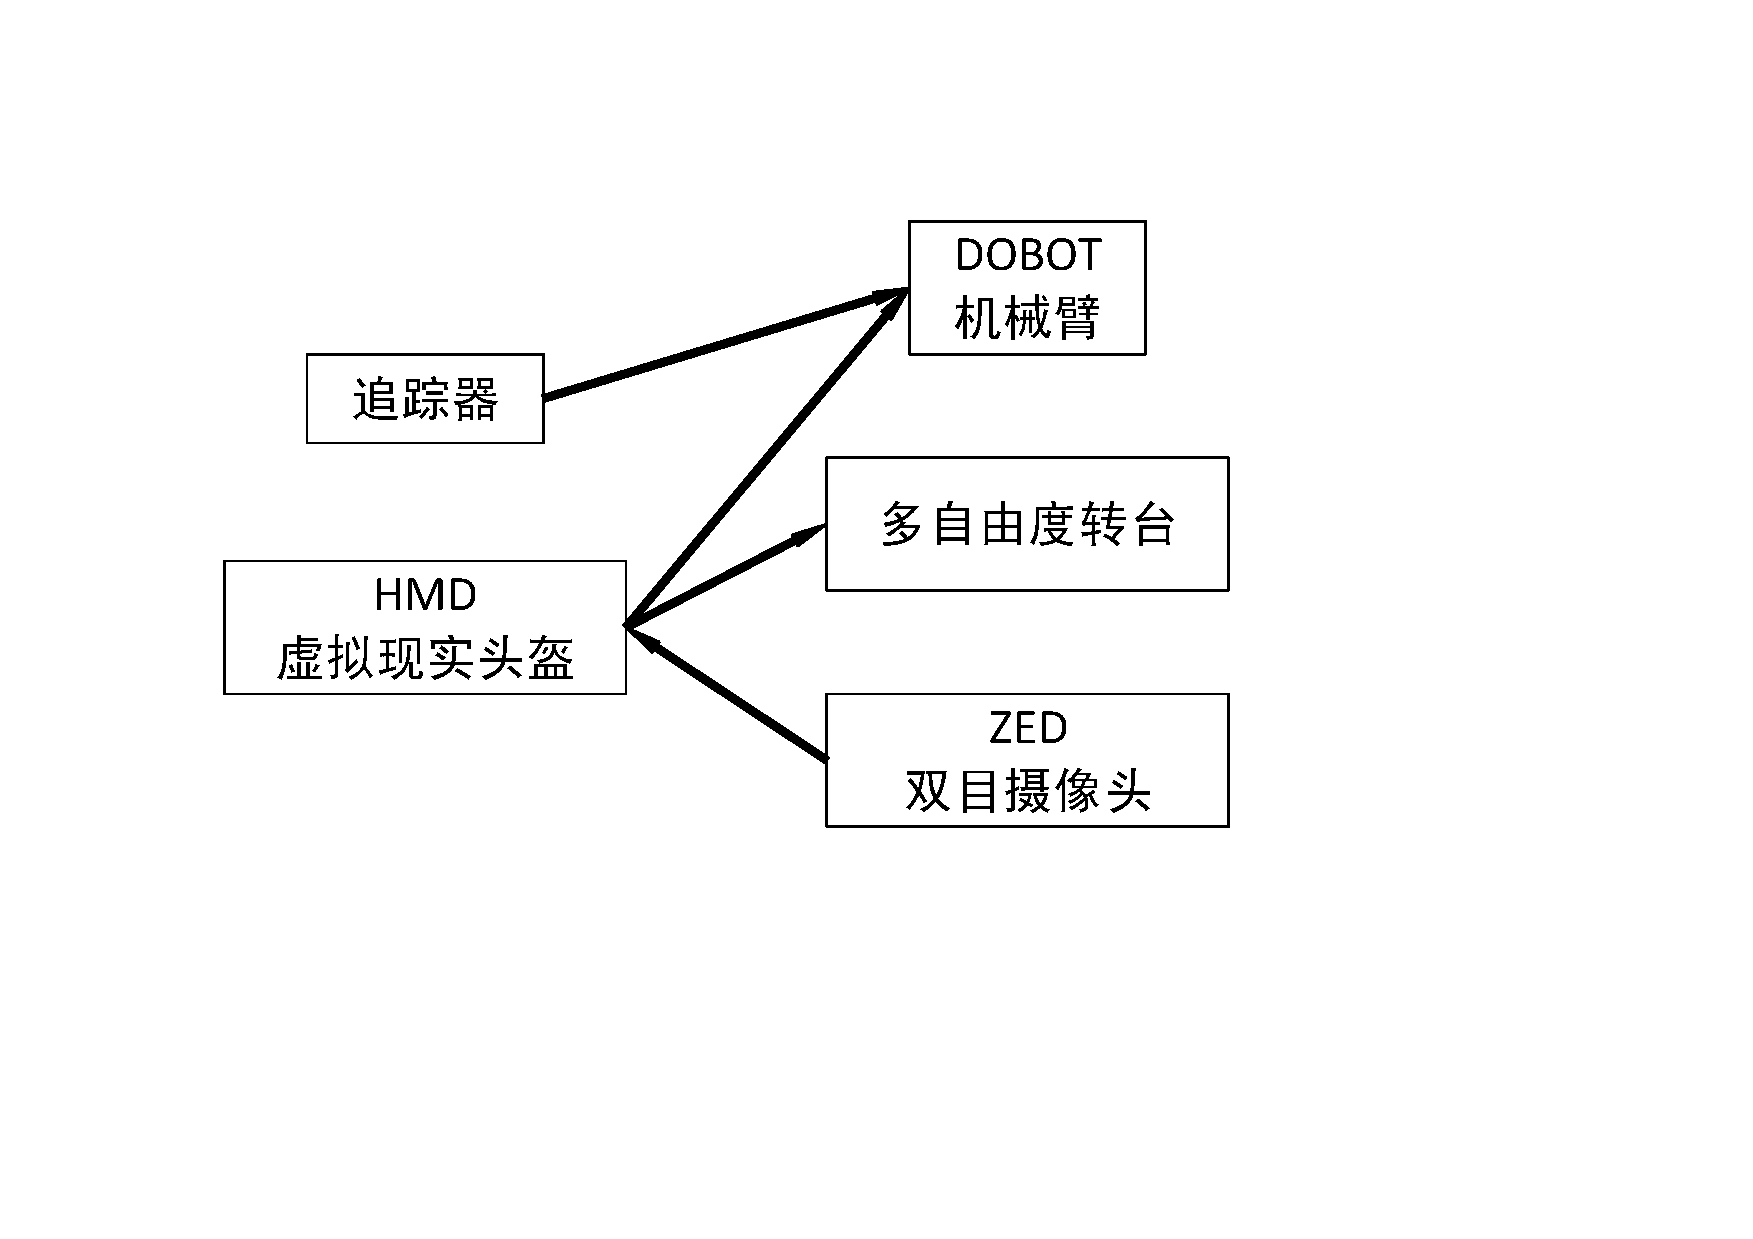
\includegraphics[width=12cm]{logic.pdf}
\caption{数据流向示意} 
\label{logic}
\end{figure}

下面分三部分介绍技术细节。

\section{实时图像采集与显示系统}
ZED双目摄像头两个目采集到的图像分别投射到Vive头盔的两个显示屏中。ZED双目摄像头搭载在由两个数字舵机组成的双自由度平台上,以保证双目朝向与人眼朝向实时一致。

整个系统放置在4轮全向轮底盘上面, ZED双目摄像头采集到的图像,通过USB3.0发送给Nvidia Jetson TX1\footnote{\url{http://www.nvidia.cn/object/embedded-systems-dev-kits-modules-cn.html}},TX1上运行Ubuntu系统,图像在TX1上处理后,使用UV4L服务(User space Video4Linux)\footnote{\url{https://www.linux-projects.org/uv4l/}}发送到局域网。同时,Vive VR头盔的姿态数据通过HTC串流盒发送到计算机中进行处理,处理后通过蓝牙串口发送到全向轮车上面的下位机(Arduino Mega 2560),控制双自由度数字舵机做出与Vive VR头盔同步的转动,使安装在双自由度数字舵机平台上的ZED双目摄像头的指向与Vive头盔实时相同。

\section{机械臂控制系统}

\begin{figure}[htbp]
\small
\centering
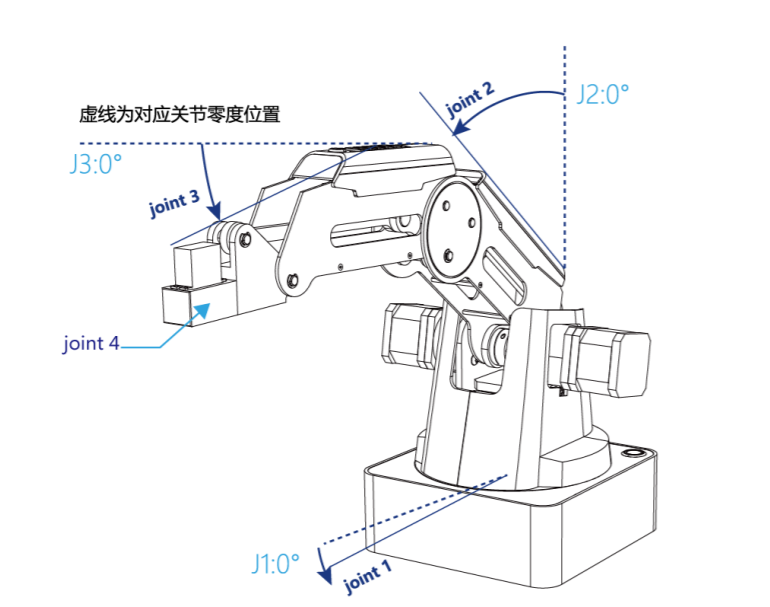
\includegraphics[width=8cm]{dobott.png}
\caption{DOBOT机械臂各自由度的示意图} 
\label{dobott}
\end{figure}

图~\ref{dobott}为Dobot各自由度的示意图,机械臂在三维空间中的移动需要用到joint1、2、3,该三个自由度简化后的模型如下图所示。

其中a,b分别为两个臂的长度,根据官方资料,$a=135mm$,$b=147mm$。$\alpha$、$\beta$、$\theta$ 为三个自由度对应的方位角。

\begin{figure}[htbp]
\small
\centering
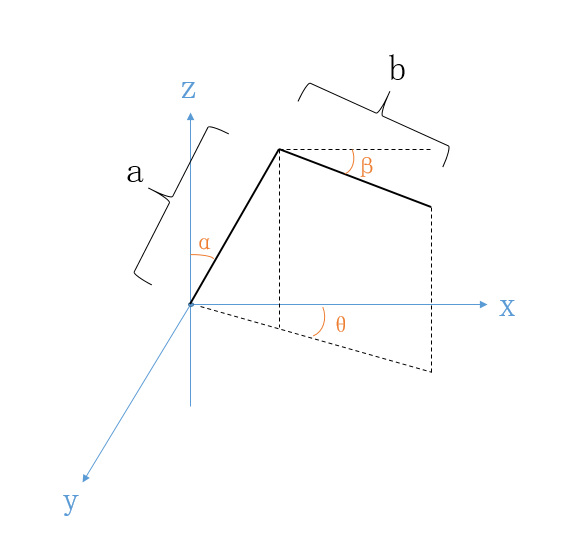
\includegraphics[width=8cm]{dobotg.png}
\caption{DOBOT机械臂末端坐标表示示意图} 
\label{dobotg}
\end{figure}

由图~\ref{dobotg}可得,末端坐标的位置$(x,y,z)$可表示为:

\begin{equation}
x=(a \times sin(\alpha)+b \times cos(\beta)) \times cos(\theta)
\end{equation}

\begin{equation}
y=(a \times sin(\alpha)+b \times cos(\beta)) \times sin(\theta)
\end{equation}

\begin{equation}
z=a*cos(\alpha)-b*cos(\beta)
\end{equation}

可见,任意一组给定的x,y,z坐标都有唯一的一组$\alpha$、$\beta$、$\theta$与之对应,只要得到方位角与坐标之间的关系即可将机械臂移动到其可触及的任意位置。

\begin{enumerate}
\item 点对点移动:
联立以上方程组,解得:
\begin{displaymath}
\alpha {\rm{ = arcsin(}}\frac{{{x^2} + {y^2} + {z^2} - {b^2}}}{{2a\sqrt {{x^2} + {y^2} + {z^2}} }}) - {\rm{arcsin(}}\frac{z}{{\sqrt {{x^2} + {y^2} + {z^2}} }})
\end{displaymath}

\begin{displaymath}
\beta {\rm{ =  - arcsin(}}\frac{{{x^2} + {y^2} + {z^2} - {a^2}}}{{2b\sqrt {{x^2} + {y^2} + {z^2}} }}) + {\rm{arccos(}}\frac{z}{{\sqrt {{x^2} + {y^2} + {z^2}} }})
\end{displaymath}

由求出的$\alpha$、$\beta$可得到
\begin{equation}
\theta {\rm{ = }}\arcsin (\frac{y}{{a \times \sin \alpha  + b \times \cos \beta }})
\end{equation}

由此可将任意一点的$(x,y,z)$坐标用机械臂三个自由度的方位角$(\alpha,\beta,\theta)$来表示,,因而可通过各关节的转动而实现点对点运动。即初始坐标为$(x_1,y_1,z_1)$,目的坐标为$(x_2,y_2,z_2)$,则可用上述方法计算出相应的$(\alpha_1,\beta_1,\theta_1)$,$(\alpha_2,\beta_2,\theta_2)$,从而得知各关节需转动的角度。

\item 基于运动方向的移动
机械臂在$(x,y,z)$坐标系中各轴的速度分量也可由$(\alpha,\beta,\theta)$坐标系中的角速度表示:
\begin{displaymath}
\begin{array}{l}
{v_x} = \frac{{dx}}{{dt}} = \frac{{\delta x}}{{\delta \alpha }}\frac{{\delta \alpha }}{{\delta t}} + \frac{{\delta x}}{{\delta \beta }}\frac{{\delta \beta }}{{\delta t}} + \frac{{\delta x}}{{\delta \theta }}\frac{{\delta \theta }}{{\delta t}} \\= a\cos \alpha \cos \theta {w_\alpha } - b\sin \beta \cos \theta  - (a\sin \alpha  + b\cos \beta )\sin \theta {w_\theta }\\

\end{array}
\end{displaymath}
\begin{displaymath}
{v_y} = a\cos \alpha \sin \theta {w_\alpha } - b\sin \beta \sin \theta  + (a\sin \alpha  + b\cos \beta )\cos \theta {w_\theta }
\end{displaymath}
\begin{displaymath}
{v_z} =  - a\sin \alpha {w_\alpha } - b\cos \beta {w_\beta }
\end{displaymath}
用矩阵形式表示,即:
\begin{equation}
\left[ {\begin{array}{*{20}{c}}
	{{v_x}}\\
	{{v_y}}\\
	{{v_z}}
	\end{array}} \right] = \left[ {\begin{array}{*{20}{c}}
	{a\cos \alpha \cos \theta }&{ - b\sin \beta \cos \theta }&{ - (a\sin \alpha  + b\cos \beta )\sin \theta }\\
	{a\cos \alpha \sin \theta }&{ - b\sin \beta \sin \theta }&{(a\sin \alpha  + b\cos \beta )\cos \theta }\\
	{ - a\sin \alpha }&{ - b\cos \beta }&0
	\end{array}} \right]\left[ {\begin{array}{*{20}{c}}
	{{w_\alpha }}\\
	{{w_\beta }}\\
	{{w_\theta }}
	\end{array}} \right]
\end{equation}

简写为$\overrightarrow {V}  = {A}\overrightarrow w $

由于任意时刻机械臂都有确定的方位角,故$A$为已知量,因而给定一组想要得到的$(v_x,v_y,v_z)$,则可通过计算$\overrightarrow w=A^-1\overrightarrow {V}$得到对应的角度。
\end{enumerate}




\section{NAO机器人控制系统}
项目中为了控制机器人的手臂,采用逆运动学的理论,通过机器人手臂的端点结合手臂的参数来计算关节必要的旋转值来进行动作。由于NAO机器人手臂(不包括手指部分)的自由度是5个,因此在仅要设置手指尖端的目标坐标点的情况下,会出现手臂姿态不唯一的情况。通过筛选使得手臂各个关节与端点的坐标实现一一对应。

\begin{figure}[htbp]
\small
\centering
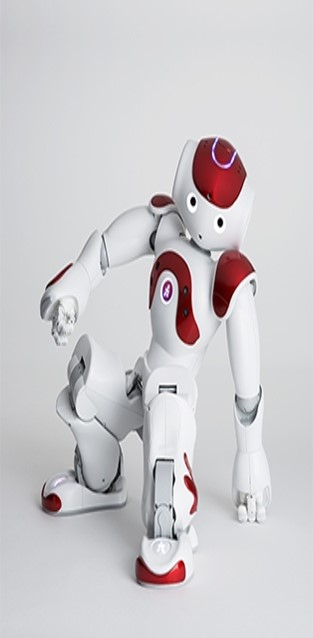
\includegraphics[width=8cm]{NAO.jpg}
\caption{NAO机器人} 
\end{figure}

对于机器人的姿态设定、手臂末端的设定涉及到机器人的控制理论。每个关节有相应的标准坐标系来解读链接和位置以及决定关节转换的基本程序。从参考点开始到第一个关节,再最终到最后一个关节完成转换后可以得到机械臂的转换矩阵。利用这个转换矩阵可以根据手臂末端的目标位置得到每个关节的转动参数。

我们主要采用Denavit Hartenberg (DH)来进行运动学的计算。根据厂家提供的机器人的手臂参数(如长度等),得到每个关节n的转换矩阵$A_n$

\begin{equation}
{{A}_n} = \left[ {\begin{array}{*{20}{c}}
	{{C_{{\theta _n}}}}&{ - {S_{{\theta _n}}}{C_{{\alpha _n}}}}&{{S_{{\theta _n}}}{S_{{\alpha _n}}}}&{{a_n}{C_{{\theta _n}}}}\\
	{{S_{{\theta _n}}}}&{{C_{{\theta _n}}}{C_{{\alpha _n}}}}&{ - {C_{{\theta _n}}}{S_{{\alpha _n}}}}&{{a_n}{S_{{\theta _n}}}}\\
	0&{{S_{{\alpha _n}}}}&{{C_{{\alpha _n}}}}&{{d_n}}\\
	0&0&0&1
	\end{array}} \right]
\end{equation}

其中${C_{{\theta _n}}} = \cos ({\theta _n})$,${S_{{\theta _n}}} = \sin ({\theta _n})$, ${{\theta }_{n}}$为官方给出的旋转角,$a_n$为两个关节参考坐标系中坐标轴交界口的距离,$d_n$为两个关节在同意旋转轴上的距离,这些数据都可以在NAO的数据手册中查询到。

为了根据目的点的坐标分离方程,以得到各个关节的转动值,我们将变换矩阵"An"的逆矩阵相乘于关系方程的左边来取得计算角度值的元素。右手包含五个关节,从上到下分别是肩膀关节(RShoulderPitch,RShoulderRoll 两个),手肘关节(elbow RElbowRoll,RElbowYaw 两个),和手腕关节(RWristYaw)。因此,表示从肩膀到手腕各关节的转动矩阵为${}_{S}^{W}{T}$

\begin{equation}
{}_{s}^{\rm{w}}{T = }{{A}_{1}} \times {{A}_{2}} \times {{A}_{3}} \times {{A}_{4}} \times {{A}_{5}}
\end{equation}

\begin{equation}
	A = {A_1} \times {A_2} \times {A_3} \times {A_4} \times {A_5} = \left[ {\begin{array}{*{20}{c}}
		{{r_{11}}}&{{r_{12}}}&{{r_{13}}}&{{p_x}}\\
		{{r_{21}}}&{{r_{22}}}&{{r_{23}}}&{{p_y}}\\
		{{r_{31}}}&{{r_{32}}}&{{r_{33}}}&{{p_z}}\\
		0&0&0&1
		\end{array}} \right]
\end{equation}

然后我们通过逐步乘以 $ A_i^{-1} $ 的方式得到各个关节的变换矩阵A,进而可以通过以下公式得到每个关节的转动参数。

\begin{equation}
{Pos\_w = A} \times {Pos\_s}
\end{equation}

由以上方程并结合NAO的链接关节变量数据(在NAO官网上提供),我们可以根据目的点得到每个关节点旋转的角度,从而达到基于逆运动学控制机器人的机械臂。


\chapter{展望}

\section{改进}
下一阶段,我们将从以下几个方面改进该系统:
\begin{itemize}
    \item 给NAO编写行走程序,加入闭环反馈,从软件层面提高NAO的稳定性
    \item 采集每次操作的数据,使用增强学习训练机器人自主地执行任务。
    \item 加上手势识别元件实现机器人手部的动作,进一步完善机器人的功能。
\end{itemize}

\section{应用}

随着科技技术的不断发展,人类正向许多未知的领域前进,而这个过程注定危险重重。如深水、深地层、外层空间、强放射、高真空等新的生产和作业领域。由于自动控制尚无法独立执行复杂任务,此系统可以帮助技术人员远程执行任务,而无需复杂的遥操作培训和练习。

例如,随着航天事业的发展,如今空间站中的宇航员可能需要完成各种危险的出舱任务。在这种情况下,就可以采用本技术,在太空舱中遥控机器人在舱外完成本来艰巨危险的任务。(如图~\ref{arm})

未来此技术可以用于航天,拆弹,救援,深海作业,远程交互等领域。

\begin{figure}[htbp]
\small
\centering
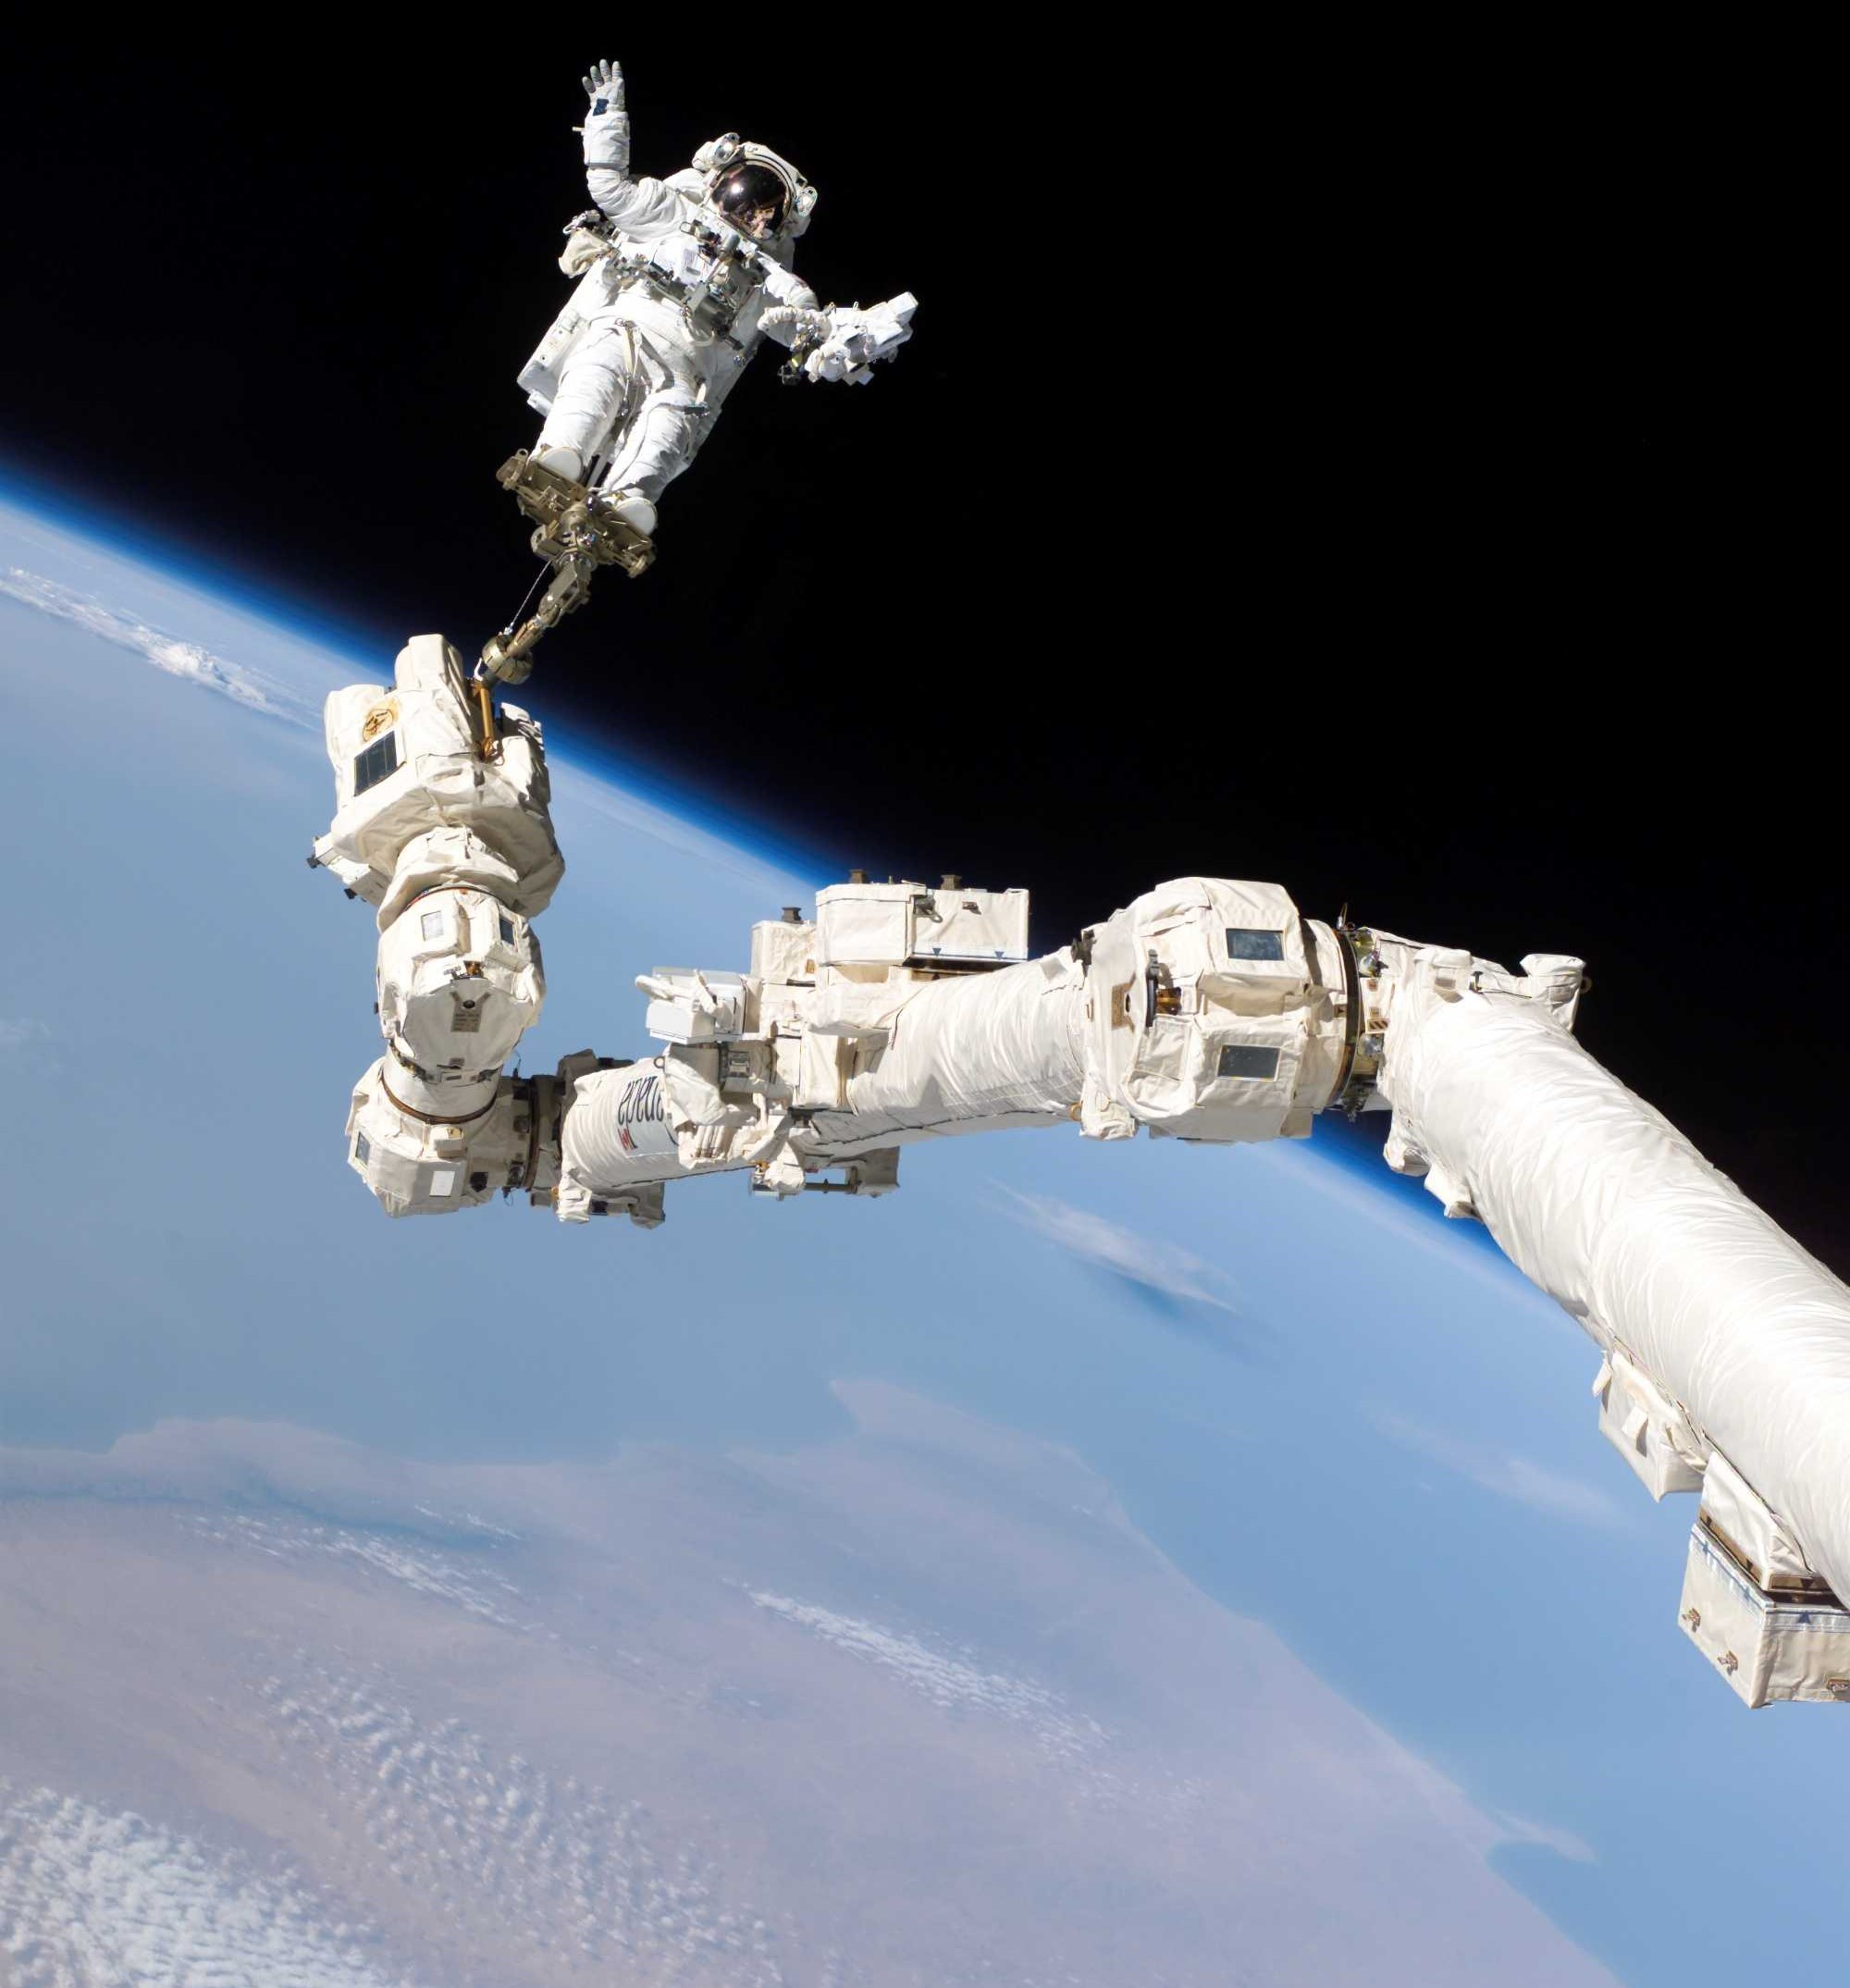
\includegraphics[width=8cm]{robotic_arm_large.jpg}
\caption{国际空间站的机械臂(可以帮助宇航员在太空中举起大型物体)} 
\label{arm}
\end{figure}

